\documentclass[a4paper]{article}

\usepackage[english]{babel}
\usepackage[utf8x]{inputenc}
\usepackage{amsmath}
\usepackage{graphicx}
\usepackage[colorinlistoftodos]{todonotes}
\usepackage{verbatim}

\title{IST557 Project 1}
\author{Kyle,Sagnik,Wenyi}

\begin{document}
\maketitle

\begin{abstract}
We use KDD cup 2013 dataset in this project to compare different classification methods. 
\end{abstract}

\section{Introduction}

In Kdd Cup 2013, the author name disambiguation problem was framed as a binary classification task. Given a set of (author, pair) entries, we had to classify each of them as positive (the author actually wrote that paper) or negative (the author didn't write that paper). From the given dataset described below (section \ref{sec:examples}), we extracted some features, applied PCA, LDA and QDA and tested our model through cross validation.  

\section{Dataset and Features}
\label{sec:examples}

\subsection{Original Dataset}
Following content is taken from KDD cup dataset page [] and presented with modificationas as necessary. 


The provided datasets are based on a snapshot taken in Jan 2013 and contain:

An \textbf{Author dataset} (Author.csv) with profile information about 250K authors, such as author name and affiliation. The same author can appear more than once in this dataset, for instance because he/she publishes under different versions of his/her name, such as J. Doe, Jane Doe, and J. A. Doe. (see table \ref{table:author})

\begin{table}
  \caption{Author dataset}
\begin{tabular}{ |l |l |l |}
  \hline
  \textbf{Name} & \textbf{Data Type} & \textbf{Comments} \\ \hline
  Id & Int & Id of the author\\ \hline
  Name & NVarchar &  Name of the author\\ \hline
  Affiliation & NVarchar & Organization name with which the author is affiliated.  \\ \hline
\end{tabular}
\label{table:author}
\end{table}


A \textbf{Paper dataset} (Paper.csv) with data about 2.5M papers, such as paper title, conference/journal information, and keywords. The same paper may have been obtained through different data sources and hence have multiple copies in the dataset (see table \ref{table:paper}). 

\begin{table}
  \caption{Paper dataset}
\begin{tabular}{ |l |l |l |}
  \hline
 \textbf{Name} & \textbf{Data Type} & \textbf{Comments} \\ \hline
  Id & Int & Id of the paper \\ \hline
  Title & NVarchar &  Title of the paper\\ \hline
  Year & Int & Year of the paper  \\ \hline
  ConferenceId & Int & Conference Id in which paper was published\\ \hline
  JournalId & Int & Journal Id in which paper was published \\ \hline
  Keywords & Nvarchar & Keywords of the paper \\ \hline  
\end{tabular}
\label{table:paper}
\end{table}

A corresponding \textbf{Paper-Author dataset} (PaperAuthor.csv) with (paper ID, author ID) pairs. The Paper-Author dataset is noisy, containing possibly incorrect paper-author assignments that are due to author name ambiguity and variations of author names (see table \ref{table:paperauthor}).

\begin{table}
  \caption{Paper-Author dataset}
\begin{tabular}{ |l |l |l |}
  \hline
 \textbf{Name} & \textbf{Data Type} & \textbf{Comments} \\ \hline
  PaperId & Int & Paper Id\\ \hline
  AuthorId & Int & Author Id\\ \hline
  Name & Nvarchar & Author Name (as written on paper)\\ \hline
  Affiliation & Nvarchar & Author Affiliation (as written on paper)\\ \hline
\end{tabular}
\label{table:paperauthor}
\end{table}

Since each paper is either a conference or a journal, \textbf{additional metadata} (see table ) about conferences and journals is provided where available (Conference.csv, Journal.csv) (see table \ref{table:confjournal}).

\begin{table}
  \caption{Paper-Author dataset}
\begin{tabular}{ |l |l |l |}
  \hline
 \textbf{Name} & \textbf{Data Type} & \textbf{Comments} \\ \hline
  Id & Int & Conference Id or Journal Id \\ \hline
  ShortName & NVarchar & Short Name\\ \hline
  FullName & Nvarchar & Full Name\\ \hline
  HomePage & Nvarchar & Homepage URL of conf/journal \\ \hline
\end{tabular}
\label{table:confjournal}
\end{table}

\textbf{Co-authorship can be derived from the Paper-Author dataset}.

 

Papers that authors have "confirmed" (acknowledging they were the author) or deleted (meaning they were not the author) have been split into Train, Validation, and Test sets based on the author's Id. 


\subsection{Extracted Features}

For each ($a_i,p_j$) pair, we extracted following features:
\begin{enumerate}
\item Number of papers $a_i$ has published in the journal $p_j$ was published in.
\item Number of papers $a_i$ has published in the conference $p_j$ was published in.
\item Number of papers $a_i$ has published.
\item Number of authors in $p_j$.
\item Suppose co-authors of $a_i$ for $p_j$ are $A_k | k \in (1:n)$. We created a vector P such that $P_{k}$= number of papers $a_i$ co-authored with $A_k$. We used sum, min, max, standard deviation and mean of the vector as separate features.
\item Suppose co-authors of $a_i$ for $p_j$ are $A_k | k \in (1:n)$. We created a coauthorship vector C where C[k]= Number of conferences/journals $a_i$ and $A_k$ publish together. We used mean, standard deviation, minimum, max and sum of this vector (C) as separate features.  
\end{enumerate}

Therefore, our feature space is 14 dimensional. 

\section{}

\begin{comment}
\subsection{Tables and Figures}


Use the table and tabular commands for basic tables --- see Table~\ref{tab:widgets}, for example. You can upload a figure (JPEG, PNG or PDF) using the files menu. To include it in your document, use the includegraphics command as in the code for Figure~\ref{fig:frog} below.

% Commands to include a figure:
\begin{figure}
\centering
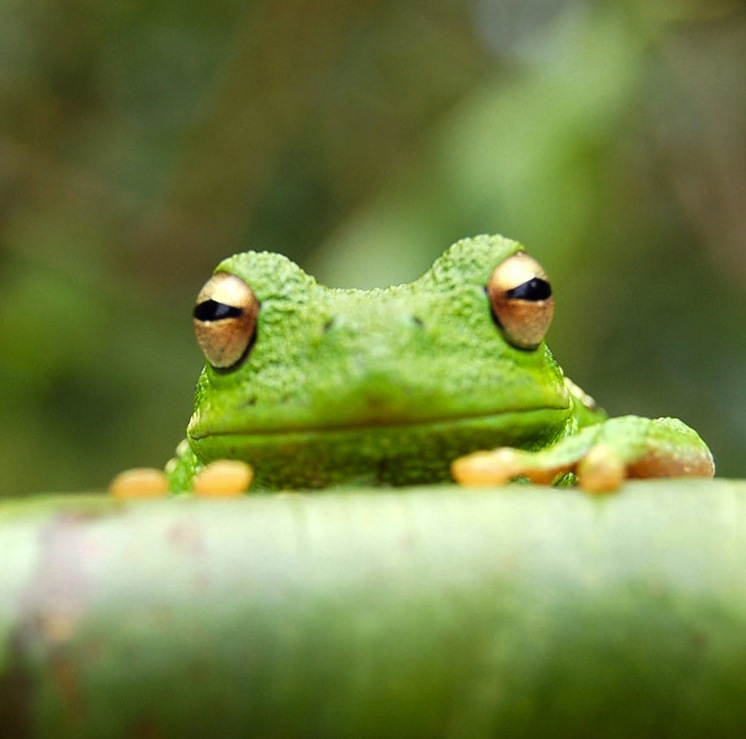
\includegraphics[width=0.5\textwidth]{frog.jpg}
\caption{\label{fig:frog}This is a figure caption.}
\end{figure}

\begin{table}
\centering
\begin{tabular}{l|r}
Item & Quantity \\\hline
Widgets & 42 \\
Gadgets & 13
\end{tabular}
\caption{\label{tab:widgets}An example table.}
\end{table}

\subsection{Mathematics}

\LaTeX{} is great at typesetting mathematics. Let $X_1, X_2, \ldots, X_n$ be a sequence of independent and identically distributed random variables with $\text{E}[X_i] = \mu$ and $\text{Var}[X_i] = \sigma^2 < \infty$, and let
$$S_n = \frac{X_1 + X_2 + \cdots + X_n}{n}
      = \frac{1}{n}\sum_{i}^{n} X_i$$
denote their mean. Then as $n$ approaches infinity, the random variables $\sqrt{n}(S_n - \mu)$ converge in distribution to a normal $\mathcal{N}(0, \sigma^2)$.

\subsection{Lists}

You can make lists with automatic numbering \dots

\begin{enumerate}
\item Like this,
\item and like this.
\end{enumerate}
\dots or bullet points \dots
\begin{itemize}
\item Like this,
\item and like this.
\end{itemize}

We hope you find write\LaTeX\ useful, and please let us know if you have any feedback using the help menu above.
\end{comment}
\end{document}
